\documentclass[11pt]{article}
\usepackage[toc,page]{appendix}
\usepackage{amsmath, amssymb}
\usepackage[utf8]{inputenc}
\usepackage[T1]{fontenc}
\usepackage[style=apa,backend=biber]{biblatex}
%\usepackage{biblatex}
\addbibresource{references.bib}
\usepackage{graphicx}
\usepackage{tikz}
\usetikzlibrary{automata,positioning,shapes.geometric, arrows.meta, fit, backgrounds, calc, chains}
\graphicspath{./images/Easy_Pictures/SMR_MULT_Repackaging}%\usepackage{kpfonts}
\usepackage{float}
\usepackage[margin=1in]{geometry}
\usepackage{cancel}
\usepackage{epsfig}
\usepackage{tikz-3dplot}
\usepackage{darkmode}
\usepackage{dirtytalk}
\usepackage{longtable,booktabs,array}
\usepackage{calc} % for calculating minipage widths
\usepackage[utf8]{inputenc}
\usepackage[T1]{fontenc}
\usepackage{xcolor}
\usepackage{listings}


\usepackage{etoolbox}
\usepackage{hyperref}
\hypersetup{
    colorlinks=true,
    linkcolor=blue,
    filecolor=magenta,      
    urlcolor=cyan,
    pdftitle={Hermeneutic Calculator},
    citecolor=blue,
    }


\urlstyle{same}

\lstdefinestyle{htmlStyle}{
    language=HTML,
    basicstyle=\ttfamily\small,
    keywordstyle=\color{blue}\bfseries,
    commentstyle=\color{gray}\itshape,
    stringstyle=\color{red},
    breaklines=true,
    frame=single,
    numbers=left,
    numberstyle=\tiny\color{gray},
    columns=fullflexible,
}
\lstdefinelanguage{HTML}{
  keywords={<!DOCTYPE, html, head, title, body, h1, h2, h3, p, div, span, a, img, ul, li, table, tr, td, th, style, link, script},
  sensitive=true,
  comment=[l]{//},
  morecomment=[s]{/*}{*/},
  morestring=[b]',
  morestring=[b]"
}
\lstset{style=htmlstyle, language=html}
% Updated to explicitly pass the language option
%\lstinputlisting[style=htmlstyle, language=html]{./html/example.html}
%\usepackage{tocloft}

% Optional: define some custom colors
\definecolor{sliceRed}{RGB}{225,224,91} % matching "varyellow" from your code
\definecolor{linkYellow}{RGB}{255,215,0}  % a golden yellow
\tdplotsetmaincoords{70}{110}

\title{Addition Strategies: Adding Bases and Adding Ones}
\author{Compiled by: Theodore M. Savich}


\begin{document}
\maketitle
\subsection*{Transcript}
Strategy descriptions and examples adapted from \textcite{HackenbergCourseNotes}. The video for this student's strategy was not a CGI video and has been removed from publicly accessible databases. 

It involved a student named Sarah, who solved 65+25. She said the following:

\textbf{Sarah's solution:} ''I used decomposing, I broke 65 into 60 and five. I broke 25 into 20 and five. I added the 60 and the 20 and I got 80. I added the 5 to 5 and I got ten. I connected the 5 to the 80 and I got 90.''


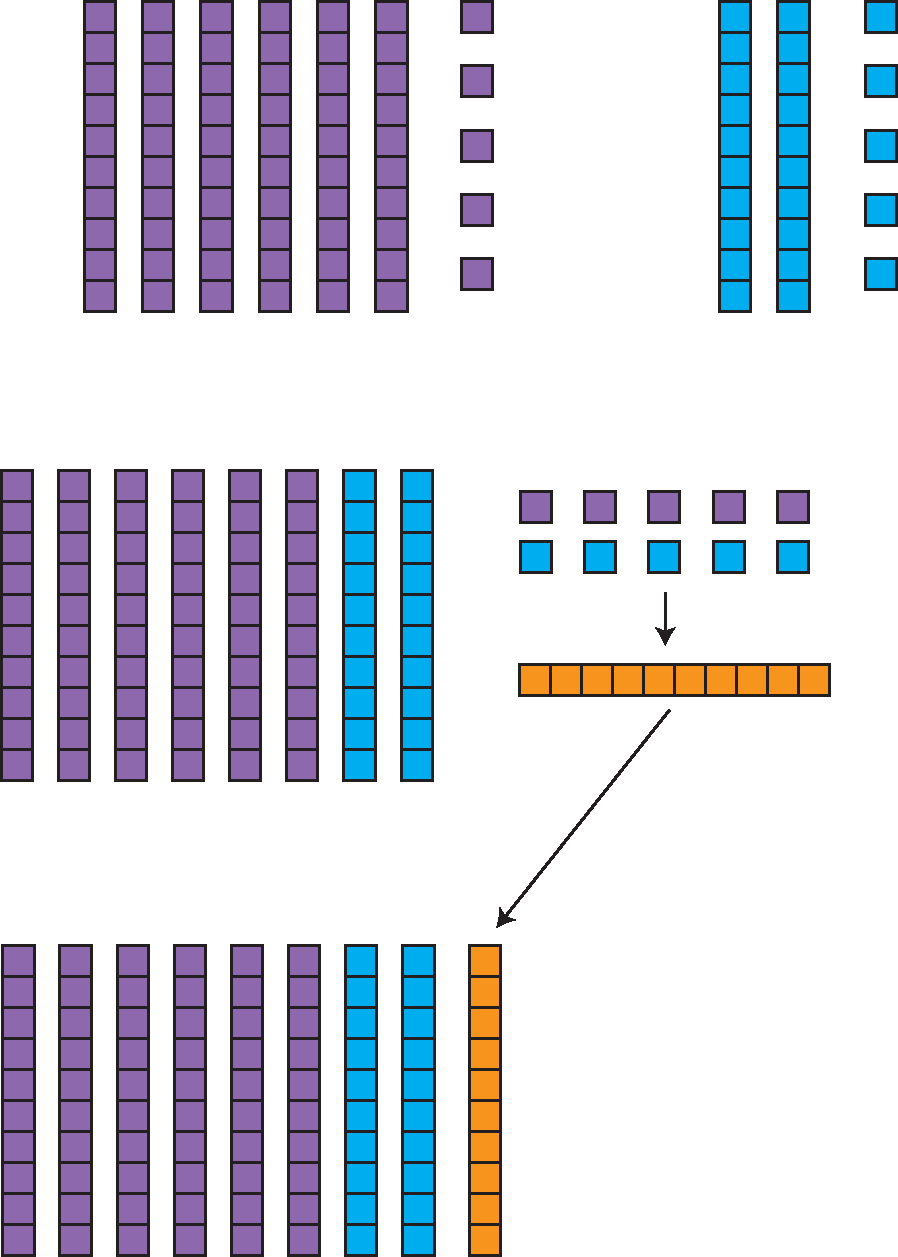
\includegraphics[width=.8\textwidth]{images/Easy_Pictures/SAR_ADD_ABAO/PDF/SAR_ADD_ABAO.pdf}

\noindent \textbf{Notation Representing Sarah's Solution:}

\begin{align*}
65 + 25 &= \Box \\
60 + 20 &= 80\\
5 + 5  &= 10\\
80+10 &= 90
\end{align*}

\subsubsection*{Description of Strategy}
\begin{itemize}
    \item \textbf{Objective:} Split both addends into bases and ones, add bases together and ones together, then combine the partial sums.
    \item \textbf{Example:} \(65 + 25\)
    \begin{itemize}
        \item Split: \(65 = 60 + 5\), \(25 = 20 + 5\).
        \item Add bases: \(60 + 20 = 80\).
        \item Add ones: \(5 + 5 = 10\).
        \item Combine: \(80 + 10 = 90\).
    \end{itemize}
\end{itemize}

\subsubsection*{Automaton Type}
\textbf{Pushdown Automaton (PDA)}: Needed to handle composition-over when adding ones.

\subsubsection*{Formal Description of the Automaton}

We define the PDA as the 7-tuple
\[
M = (Q,\, \Sigma,\, \Gamma,\, \delta,\, q_{0/accept},\, Z_0,\, F)
\]
where:
\begin{itemize}
    \item \(Q = \{q_{0/accept},\, q_1,\, q_2,\, q_3,\, q_4,\, q_5\}\) is the set of states.
    \item \(\Sigma = \{0,1,2,3,4,5,6,7,8,9,+\}\) is the input alphabet.
    \item \(\Gamma = \{Z_0\} \cup \{c \mid c \in \mathbb{N}\}\) is the stack alphabet, where \(Z_0\) is the initial stack symbol and a symbol \(c\) represents a composition-over.
    \item \(q_{0/accept}\) is the start state (which is also the accept state).
    \item \(Z_0\) is the initial stack symbol.
    \item \(F = \{q_{0/accept}\}\) is the set of accepting states.
\end{itemize}

The transition function \(\delta\) is defined as follows:
\begin{enumerate}
    \item \(\delta(q_{0/accept},\, \text{``}A,B\text{''},\, Z_0) = \{(q_1,\, Z_0)\}\) \\
          (Read \(A\) and \(B\) and split each into its base (tens, hundreds, \(\ldots\)) and ones components.)
    \item \(\delta(q_1,\, \varepsilon,\, Z_0) = \{(q_2,\, Z_0)\}\) \\
          (Add the bases: compute \(A_{\text{base}} + B_{\text{base}}\).)
    \item \(\delta(q_2,\, \varepsilon,\, Z_0) = \{(q_3,\, Z_0)\}\) \\
          (Add the ones: compute \(A_{\text{ones}} + B_{\text{ones}}\).)
    \item \(\delta(q_3,\, \varepsilon,\, Z_0) = \{(q_4,\, c\,Z_0)\}\) \\
          (If the ones sum is greater than or equal to the base, push the composition \(c\) onto the stack.)
    \item \(\delta(q_4,\, \varepsilon,\, c) = \{(q_5,\, c)\}\) \\
          (Adjust the bases sum by adding the composition-over \(c\).)
    \item \(\delta(q_5,\, \varepsilon,\, Z_0) = \{(q_{0/accept},\, Z_0)\}\) \\
          (Combine the adjusted bases sum with the ones sum and output the final result.)
\end{enumerate}

\subsubsection*{Automaton Diagram for ABAO}

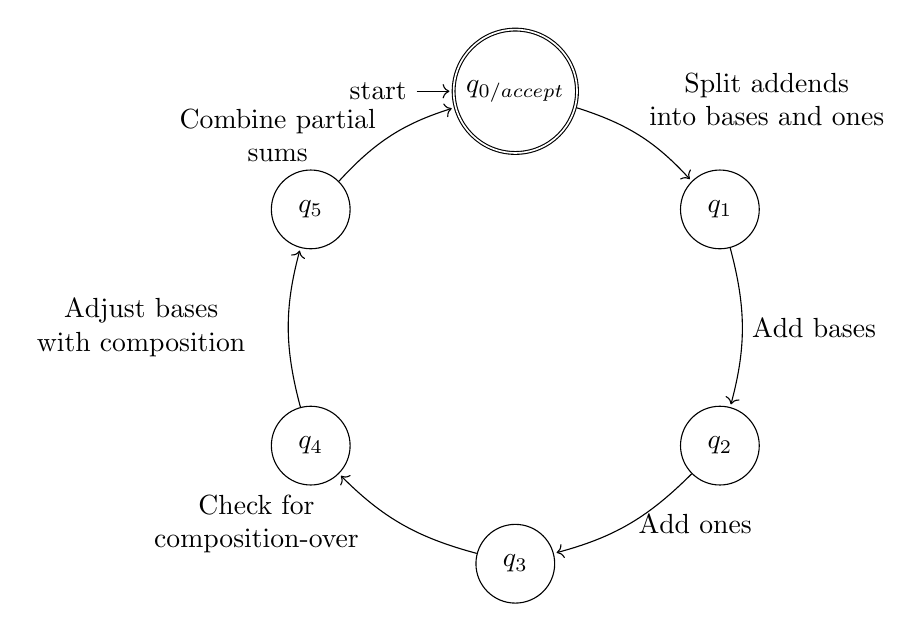
\begin{tikzpicture}[
    shorten >=1pt,
    auto,
    node distance=3cm,
    every state/.style={minimum size=1cm}
]
    % Arrange 6 states on a circle:
    % q_{0/accept} at 90°, q_1 at 30°, q_2 at -30°, q_3 at -90°, q_4 at -150°, q_5 at 150°.
    \node[state, initial, accepting] (q0) at (90:3cm) {$q_{0/accept}$};
    \node[state] (q1) at (30:3cm) {$q_1$};
    \node[state] (q2) at (-30:3cm) {$q_2$};
    \node[state] (q3) at (-90:3cm) {$q_3$};
    \node[state] (q4) at (-150:3cm) {$q_4$};
    \node[state] (q5) at (150:3cm) {$q_5$};

    % Transitions with non-overlapping labels:
    \path[->]
        (q0) edge[bend left=15] node[above right, align=center] {Split addends\\into bases and ones} (q1)
        (q1) edge[bend left=15] node[right, align=center] {Add bases} (q2)
        (q2) edge[bend left=15] node[right, align=center] {Add ones} (q3)
        (q3) edge[bend left=15] node[left=12pt, align=center] {Check for\\composition-over} (q4)
        (q4) edge[bend left=15] node[left=12pt, align=center] {Adjust bases\\with composition} (q5)
        (q5) edge[bend left=15] node[left=2pt, align=center] {Combine partial\\sums} (q0);
\end{tikzpicture}

\clearpage
\subsubsection*{HTML Implementation}
\lstinputlisting[style=htmlStyle, language=html]{./new_html/SAR_ADD_ABAO.html}

\printbibliography
\end{document}

\end{document}